% CHAPTER - Testing ---------------
\chapter{Testing}%
\label{ch:testing}
After implementing the solution developed in the various domains into the
target platforms, the system's behaviour is tested in several levels of
granularity: at the subsystem level --- unit testing, and system level ---
integrated testing. The idea is progressively test the behaviour of each
subsystem and its integration into the system.
In this chapter are presented the unit testing and integrated testing for the \gls{rfcar}.
%
\section{Unit testing}%
\label{sec:unit-testing}
    %\input{./tex/Chap/Testing/unit-testing}
    \subsection{Navigation Virtual Subsystem}%
    \label{sec:navig-virt-subsyst-implem}
    %\input{./tex/Chap/Testing/unit-testing}
    %
    \subsubsection{Control}%
    \label{sec:control-design}
    \subsubsection{System response}
The implementation of the control module was made using the modified speed algorithm mentioned and explained in \ref{sec:des-pid}.\\
The tests for this module consists in the comparison between the results obtained and simulated in \ref{sec:des-sim-res}.\\
Starting with speed reference = 1 m/s and $\theta=0~\si{rad}$:
\begin{figure}[!h]
\centering
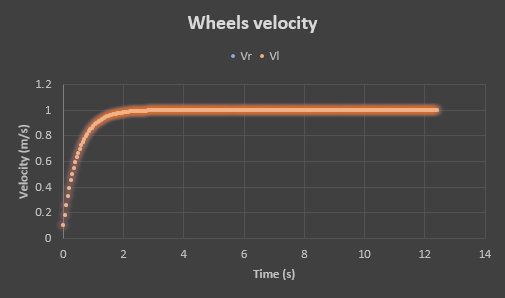
\includegraphics[width=0.7\textwidth]{./img/testv1t0.PNG}
\caption {\label{fig:test - vel0}Wheels velocity v=1m/s,$\theta = 0~\si{rad}$}
\end{figure}
In the figure \ref{fig:test - vel0} shows that the velocity of both wheels reaches the reference value in nearly 1.5 seconds, while in the simulation \ref{fig:sim1 - vel} it takes about 3 seconds. This discrepancy is due to the controller in use. The simulations  were made using the PID block provided by Simulink, while in the implementation, the controller algorithm used was as mentioned before, the modified speed algorithm. With this algorithm the behavior of the car is the same as with the traditional PID, but faster.\\
\begin{figure}[!h]
\centering
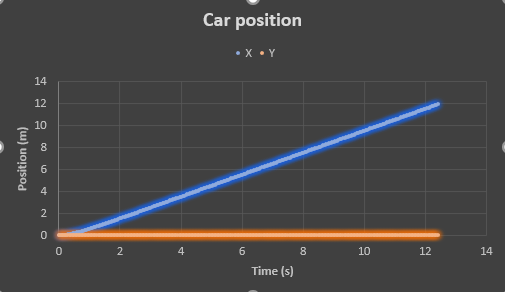
\includegraphics[width=0.7\textwidth]{./img/testx1t0.PNG}
\caption {\label{fig:test - xy0}Position v=1m/s,$\theta = 0~\si{rad}$}
\end{figure}
In the figure \ref{fig:test - xy0} it can be observed that the position of the car is the same as in the simulation \ref{fig:sim1 - pos}.\\
With speed reference = 1m/s and $\theta = 0.1~\si{rad}$:\\
\begin{figure}[!h]
\centering
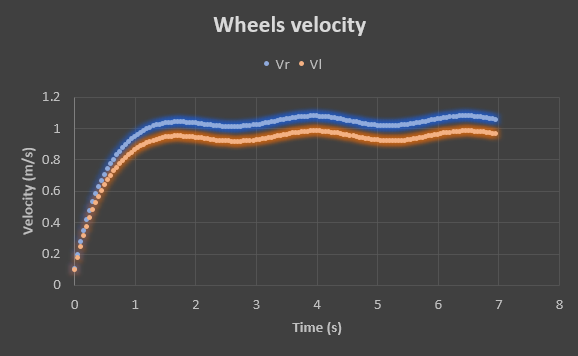
\includegraphics[width=0.7\textwidth]{./img/testv1t01.PNG}
\caption {\label{fig:test - vel01}Wheels velocity v=1m/s,$\theta = 0.1~\si{rad}$}
\end{figure}
In the figure \ref{fig:test - vel01} comparing to \ref{fig:sim2 - vel} it's possible to see that once again the time it takes to reach steady state is smaller for the reason mention before. In the implemented algorithm it's also possible to see that the steady value of the velocity of both wheels has a ripple around the reference value. \\
\begin{figure}[!h]
\centering
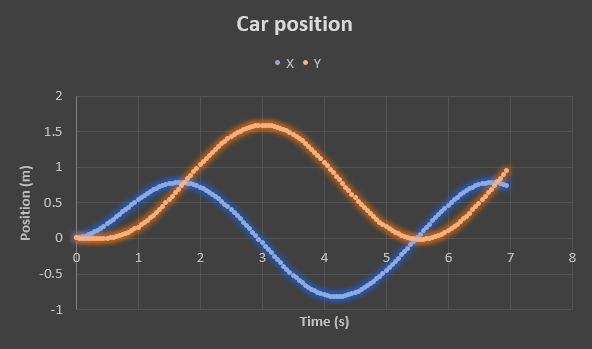
\includegraphics[width=0.7\textwidth]{./img/testx1t01.PNG}
\caption {\label{fig:test - xy01}Position v=1m/s,$\theta = 0.1~\si{rad}$}
\end{figure}
In the figure \ref{fig:test - xy01} it is present the position of the car. In comparison to the simulated \ref{fig:sim2 - pos} it is possible to see that the results are the same, thus validating the implementation.\\
\subsubsection{Obstacle Avoidance Through Odometric Sensors}
The car composed by 9 odometric sensors radially distributed, 40 degrees apart.\\
In order to test if the car can avoid obstacles, the values for the sensors were generated, and the behavior of the car was as follows:\\
\begin{figure}[!h]
\centering
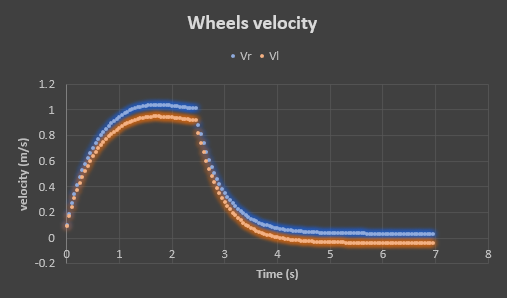
\includegraphics[width=0.7\textwidth]{./img/testodovel.PNG}
\caption {\label{fig:test - odovel}Wheels velocity}
\end{figure}

\begin{figure}[!h]
\centering
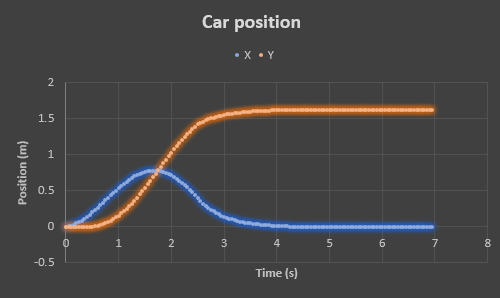
\includegraphics[width=0.7\textwidth]{./img/testodoxy.PNG}
\caption {\label{fig:test - odoxy}Car position}
\end{figure}

In the figure \ref{fig:test - odovel} it is possible to see that at t=2.5 seconds the velocity of both wheels starts decreasing until they reach a value near 0 m/s. Even though the velocity of both wheels is not exactly 0 m/s, the values are too small to break the inertia of the wheels, so the car effectively stops.
In the figure \ref{fig:test - odoxy} it is possible to see that the position of the car remains the same after the decrease of the velocity of the wheels, proving that the car is not moving.
    %
    \subsection{Physical Environment Virtual Subsystem}%
    \label{sec:phys-envir-virt-design}
    %\input{./tex/Chap/Testing/unit-testing}
    %
    %\subsection{Remote Vision Virtual Subsystem}%
    %\label{sec:remote-visi-subsyst-testing}
    \subsection{Remote Vision Virtual Subsystem}%
\label{sec:remote-visi-subsyst-testing}
In this section are presented the tests performed on the \gls{rvvs} subsystem in
the relevant domains.
%
\subsubsection{Image Acquisition}%
\label{sec:img-acq-rvvs-test}
The image acquisition system, implemented in
Section~\ref{sec:img-acq-rvvs-implem}, was tested out to assess its behaviour.

Firstly, it was selected the built-in webcam from host and attached to the guest
\gls{vm}. However,
and despite extensive troubleshooting, the bypass suggested for web
cameras\cite{webcam-bypass} was not possible for a Mac OS host. Thus, a quick
alternative was to flash a Linux \gls{os} onto a \gls{sd} card and plug it to a
Raspberry Pi 3 (available) and connect an external \gls{usb} camera to it (Fig.~\ref{fig:rasp-cam-test}).
% Raspberry Pi 3 camera test
\begin{figure}[!hbt]
\centering
    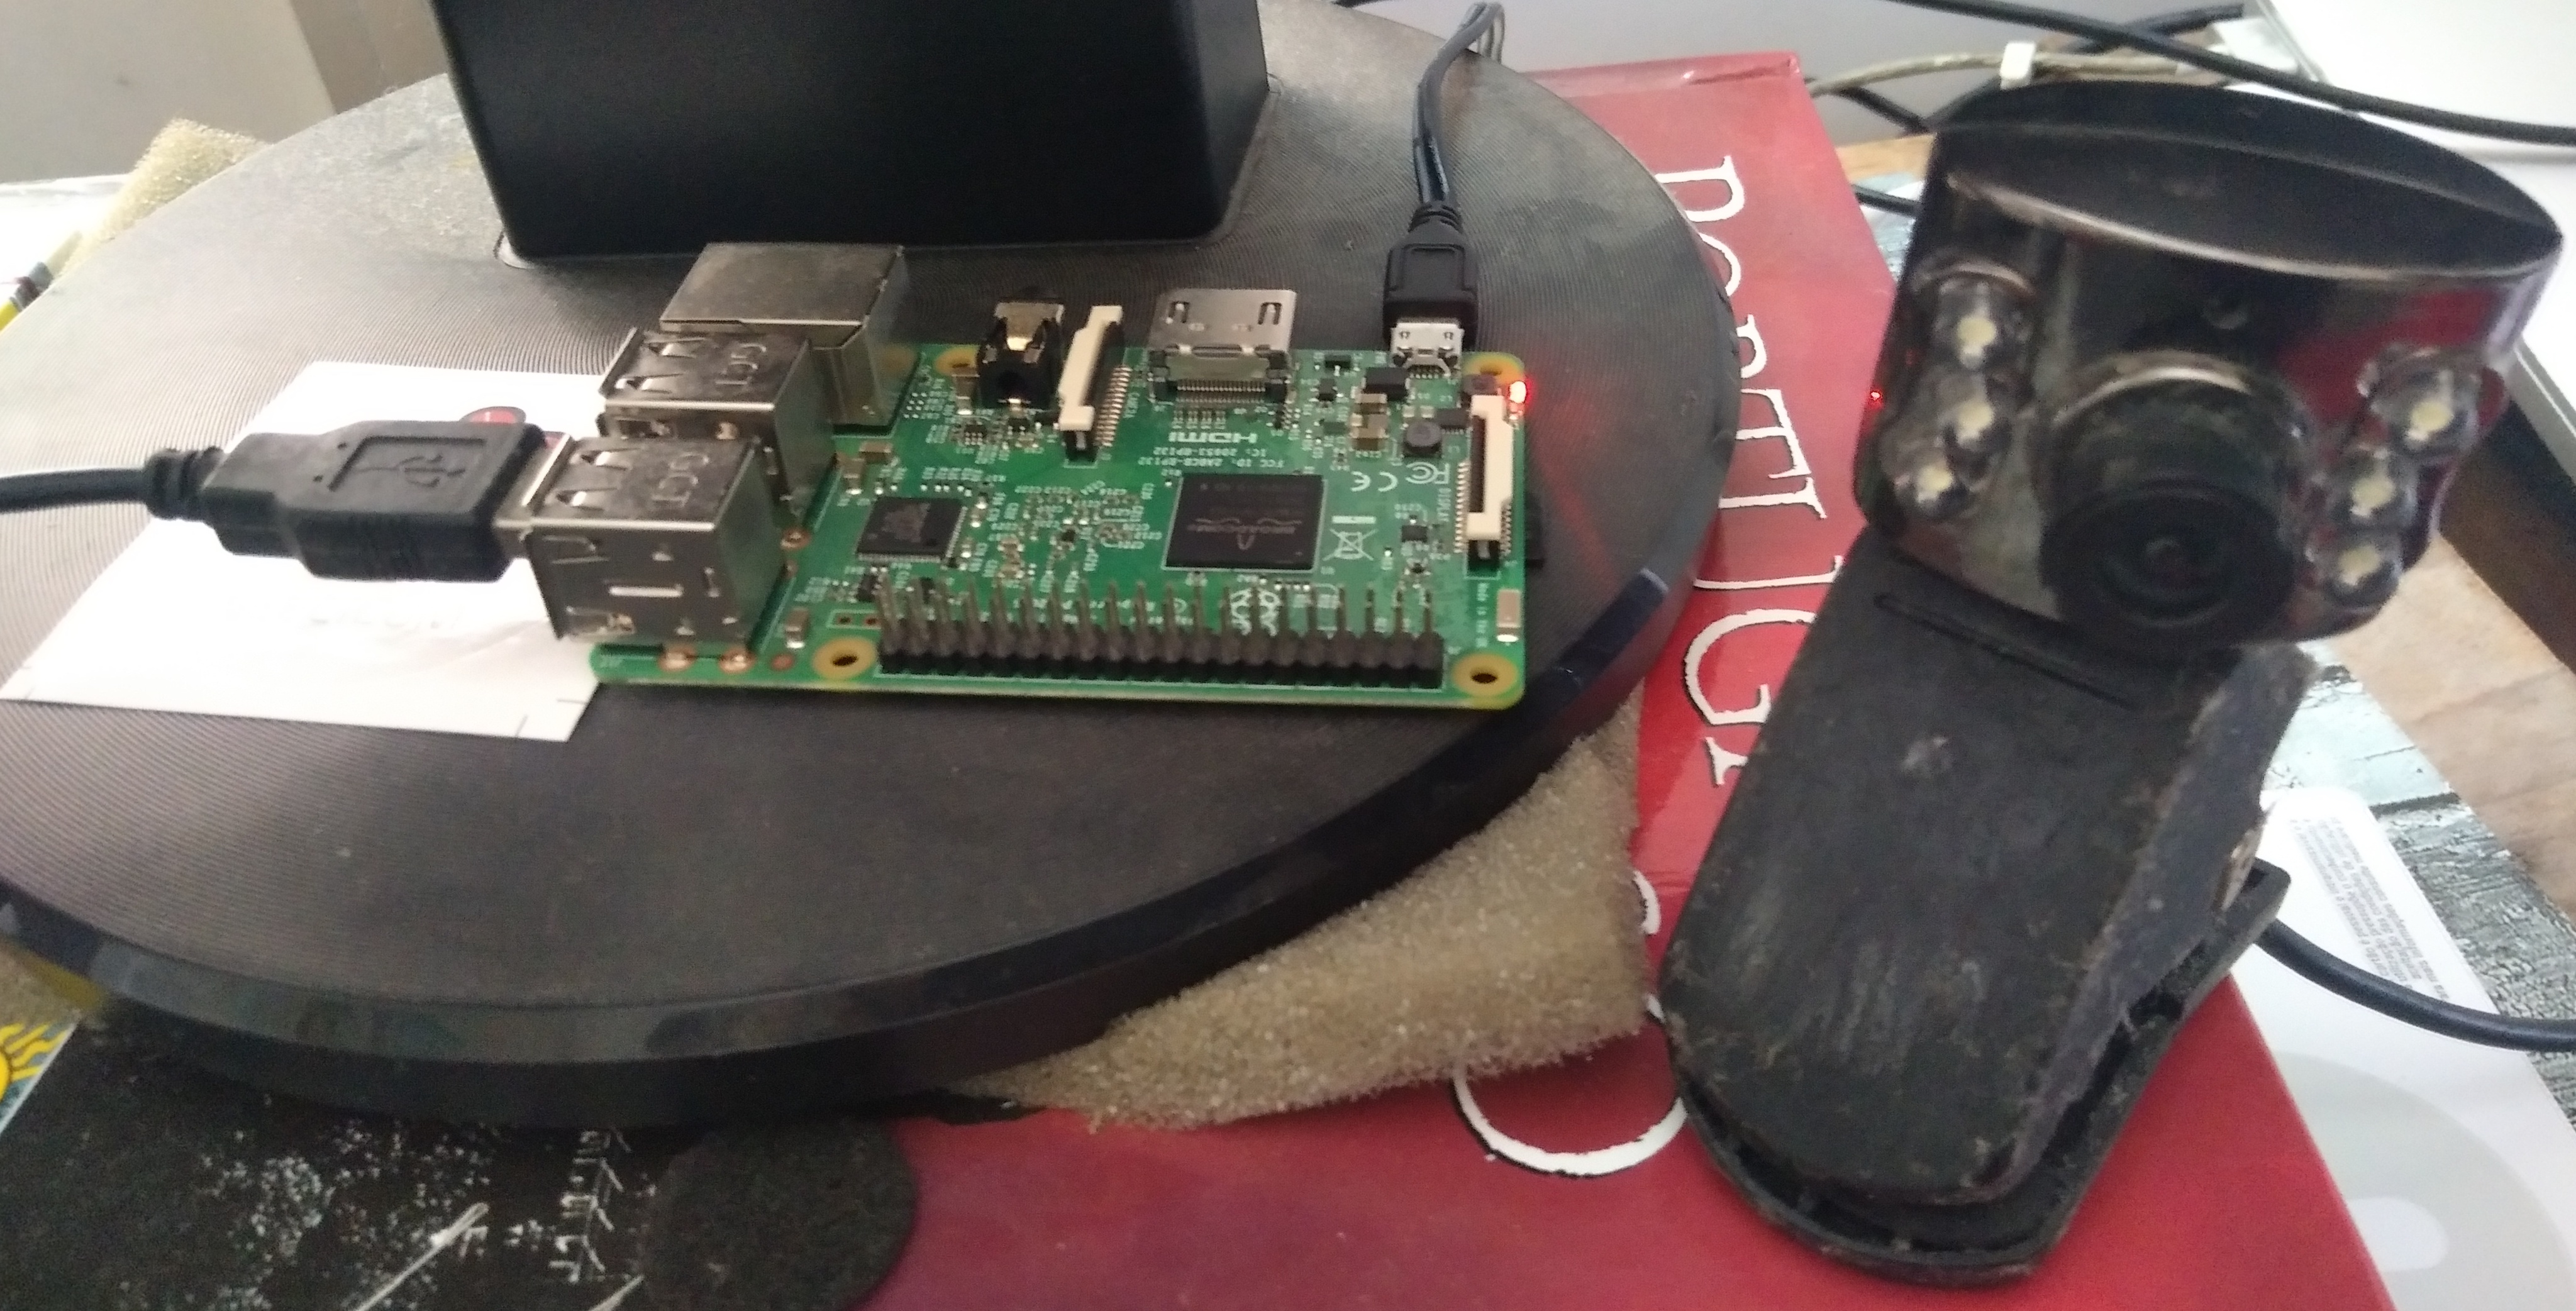
\includegraphics[width=0.6\textwidth]{./img/rasp-cam-test.jpg}
  \caption{Raspberry Pi 3 + Webcam testing setup}%
\label{fig:rasp-cam-test}
\end{figure}
%

The deployment was performed using the \gls{ssh} protocol to connect to the
Raspberry Pi and execute the necessary commands on it, and using the \gls{scp}
command that uses the \gls{sftp} protocol to transfer files between host and
guest (Listing~\ref{lst:deploy-cmds}).
\lstinputlisting[language=sh, caption={Deployment commands targetting Raspberry
Pi},label=lst:deploy-cmds,
style=customc]{./listing/ssh-scp.sh}%

The web camera was then tested using the \texttt{lsusb} command and piping the
output to a \texttt{.txt} file for further
examination. Listing~\ref{ref:lst:lsb-output} contains an excerpt of this output
where it can be observed the
webcam model (\texttt{Cubeternet WebCam}) and the \gls{usb}2.0 interface.
\lstinputlisting[language=sh, caption={Webcam information obtained via
  \texttt{lsusb} (excerpt)},label=lst:lsb-output,
style=customc]{./listing/lsusb-output.sh}%

However, this information by itself is not so useful. Additionally, and much
more importantly, one wants to check the capabilities of the device and the
supported formats. For that purpose it was used the \texttt{v4l2-ctl} utility
(Listing~\ref{lst:webcam-features}). It can be observed that the only format
supported is YUYV, which is a colour space based on one luminance component (Y')
and two chrominance components, called U(blue) projection and V(red projection),
respectively. The framerate is also fixed (30 fps), but with different
resolutions. This is very limitative, as the newer webcams support MJPEG
formats, easing video capture.
\lstinputlisting[language=sh, caption={Webcam supported image formats,
  resolutions, and framerates},label=lst:webcam-features,
style=customc]{./listing/webcam-features.sh}%

Effectively, it was executed the driver program for the webcam interface
(Listing~\ref{lst:webcam-main}), but it reported the unsupported format as
expected (Listing~\ref{lst:webcam-main-error}).
% webcam-main-error
\lstinputlisting[language=C++, caption={Webcam driver program error: unsupported
image format},label=lst:webcam-main-error,
style=customc]{./listing/webcam-main-error.sh}%

Then, it was tried out the \texttt{UYVY422} format by modifying the following
lines into Listing~\ref{lst:webcam-main}
(Listing~\ref{lst:webcam-main-modifs})
% webcam-main-error
\lstinputlisting[language=C++, caption={Webcam driver program error:
  modifications to support \texttt{UYVY422} format},label=lst:webcam-main-modifs,
style=customc]{./listing/webcam-main-modifs.cpp}%

Although an image in the \texttt{UYVY422} format was obtained, \texttt{ffmpeg}
requires tedious conversions between the packed format (\texttt{UYVY422}) to
planar one (\texttt{JPG}). Thus, an online tool was used to convert this image~\cite{conv-UYVY-jpg} into \texttt{jpg} format. In Fig.~\ref{fig:rasp-cam-test-succ} can be seen that an image was
successfully acquired.
% Raspberry Pi 3 camera test
\begin{figure}[!hbt]
\centering
    
\includegraphics[width=0.6\textwidth]{./img/webcam-test-success.jpg}
  \caption{Raspberry Pi 3 + Webcam test: success}%
\label{fig:rasp-cam-test-succ}
\end{figure}

However, this is a tedious process that could be avoided by using a different,
newer, web camera supporting additional formats and resolutions, which limited
severely the implementation and testing.
%
%%% Local Variables:
%%% mode: latex
%%% TeX-master: "../../../dissertation"
%%% End:

    %
    \subsection{Smartphone}%
    \label{sec:smartphone-testing}
    %
%
\subsubsection{Bluetooth}%
\label{sec:bluetooth-test}
After effectively changing the direction of a ball according to the accelerometer's state in the section \ref{sec:accelerometer-using-data-test}, one could only need to merge its code with the Bluetooth connection setup, so that, instead of sending plain text messages, one can transfer the acceleration values.
%
\subsubsection{Bluetooth: Smartphone-Smartphone}%
\label{sec:bluetooth-phone-phone}
%
The first test was based on testing the Bluetooth connection setup when the interface was comprised of two distinct smartphones. With that in mind, the connection was successful and the devices were able to exchange messages, as expected. Since this test was performed using the code done in another course unit no further in-depth explanations will be presented in this section as the code was fully functional.
%
\subsubsection{Bluetooth: Smartphone-NVS}%
\label{sec:bluetooth-phone-nvs}
%
An initial test was made with the \textbf{HC-05 Bluetooth module} inserted on the STM board. That approach only allows system engineers who have access to that module to fully test both Bluetooth client and server. 
%
However, to prove this new compound functionality, the device to be paired should also have Bluetooth drivers (setup) and specific hardware to use that protocol.
%
However, despite both devices having the forementioned drivers and hardware for the connection to succeed, that didn't happen. After some research on the topic, one can assume that the problem was caused by \textbf{android version mismatching}. Meaning that the \underline{HC-05 only recognised older android versions (prior to 4.2)}.
%
Fortunately, a new solution was found where one could run the server Bluetooth app in a virtual machine using, for example, COM6 port to communicate, and then redirect that port to another one (COM9) establishing the connection with the phone. In other words, the android app and bluetooth server app can be connected to different ports and still comunicate, due to the foresaid redirection represented in figure \ref{fig:port-red}. As an advantage, this method requires less hardware resources.
%
\begin{figure}[!ht]
\centering
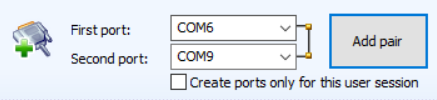
\includegraphics[width=0.5\textwidth]{img/port-red.png}
\caption{\label{fig:port-red}Port redirection}
\end{figure}
%
After turning on Bluetooth on both android (ram) and PC devices (JOAO F), as depicted in figure \ref{fig:bt_app_pc}, one could then open the android app and see in main menu its initial functionalities, figure \ref{fig:bt_intro_main}. The app manually requests Bluetooth enabling if it isn't in the beginning.
%
\begin{figure}[!ht]
\centering
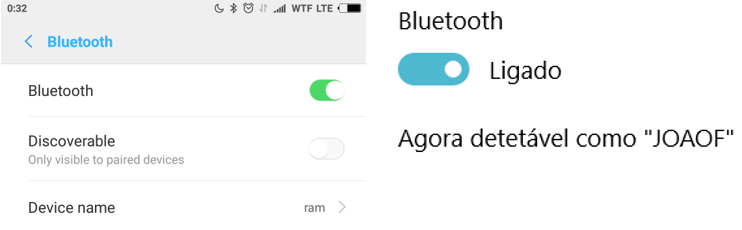
\includegraphics[width=0.9\textwidth]{img/bt_app_pc.png}
\caption{\label{fig:bt_app_pc}Smartphone as "ram" and PC as "JOAOF" with Bluetooth on}
\end{figure}
%
\begin{figure}[!ht]
\centering
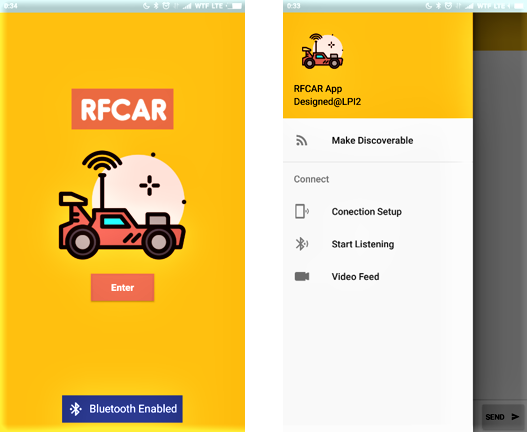
\includegraphics[width=0.5\textwidth]{img/bt_intro_main.png}
\caption{\label{fig:bt_intro_main}BTapp: Initial and main activities, accordingly}
\end{figure}
%
\begin{figure}[!ht]
\centering
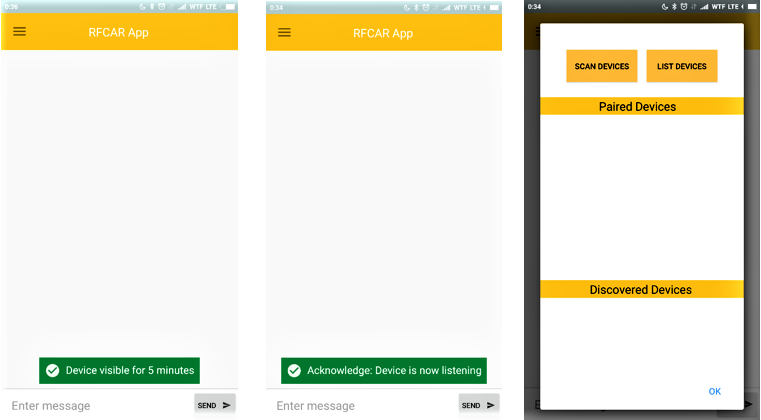
\includegraphics[width=0.7\textwidth]{img/bt_disc_list_setup.png}
\caption{\label{fig:bt_disc_list_setup}BTapp: Discoverable, Start Listening and Connection Setup activities, respectively}
\end{figure}
%
To make an initial connection from square one, the smartphone should be discoverable and then be able to start listening, so that one could configure its connection setup. To do that, the options available in the main menu were clicked in that sequence, and when making it discoverable (even if only for 300 seconds) one should accept, figure \ref{fig:bt_disc_list_setup}.
%
\begin{figure}[!ht]
\centering
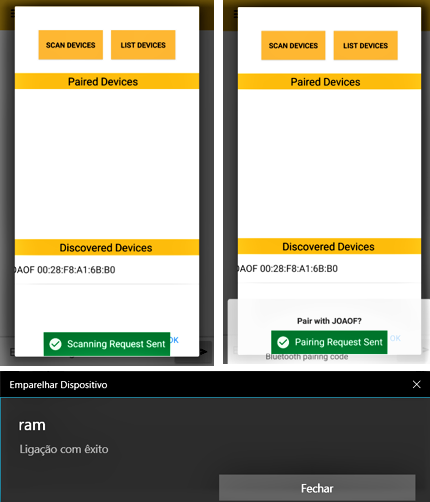
\includegraphics[width=0.4\textwidth]{img/bt_con_scan_pair_suc.png}
\caption{\label{fig:bt_con_scan_pair_suc}BTapp and PC: Pressed Scan Devices button, target device pressed and paired successfull message on PC. A PIN number given by the PC must be inserted on app to conclude the pair phase}
\end{figure}
%
\begin{figure}[!hbt]
\centering
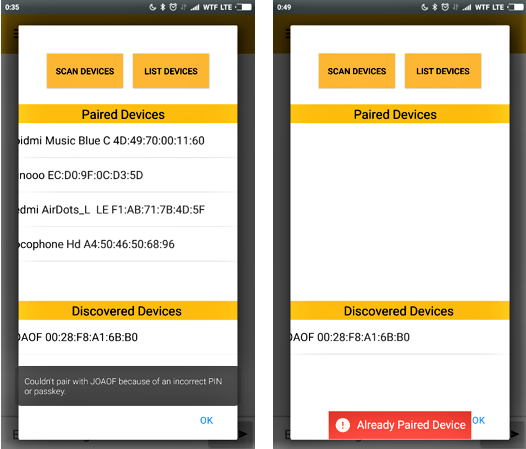
\includegraphics[width=0.4\textwidth]{img/bt_failed_pair.png}
\caption{\label{fig:bt_failed_pair}BTapp: Pair failed examples: Wrong pin number or already paired device}
\end{figure}
%
\begin{figure}[!hbt]
\centering
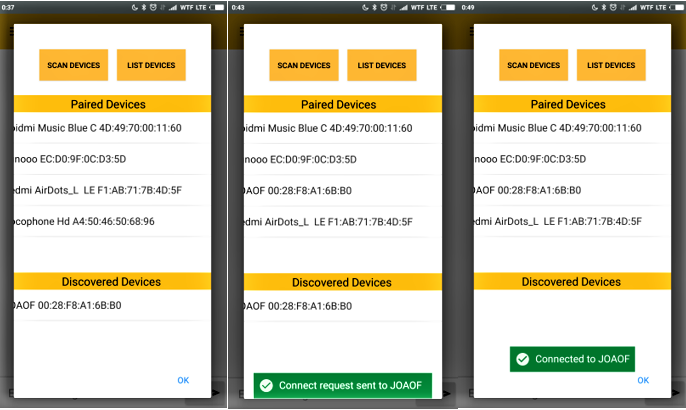
\includegraphics[width=0.5\textwidth]{img/bt_sequence_connect.png}
\caption{\label{fig:bt_sequence_connect}BTapp: Connect phases: List devices pressed, target deviced pressed and successfull display of connection establish toast}
\end{figure}
%
\begin{figure}[!hbt]
\centering
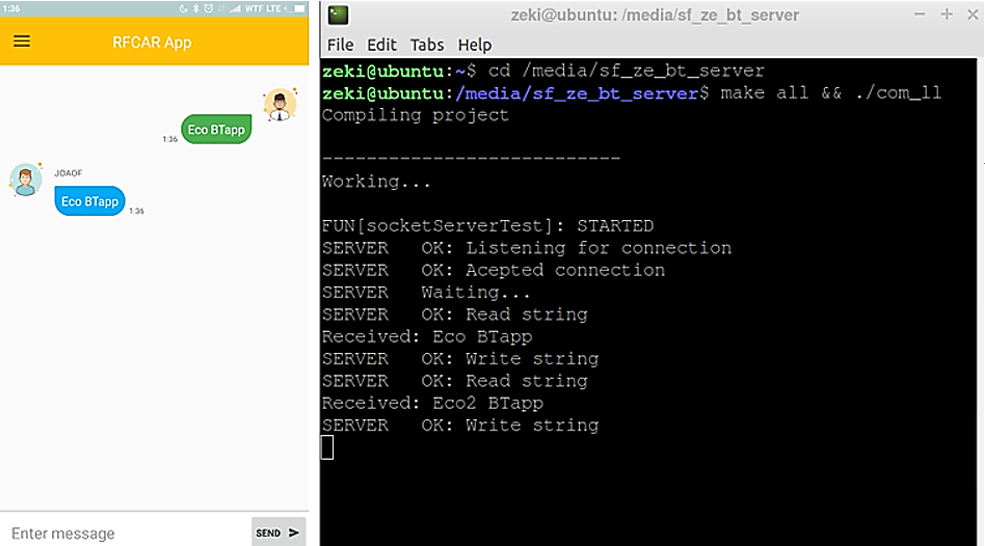
\includegraphics[width=0.5\textwidth]{img/bt_sendapp_recpc.png}
\caption{\label{fig:bt_sendapp_recpc}BTapp and PC BT server: Successfull message exchanged from android to pc and android echo}
\end{figure}
%
\begin{figure}[!hbt]
\centering
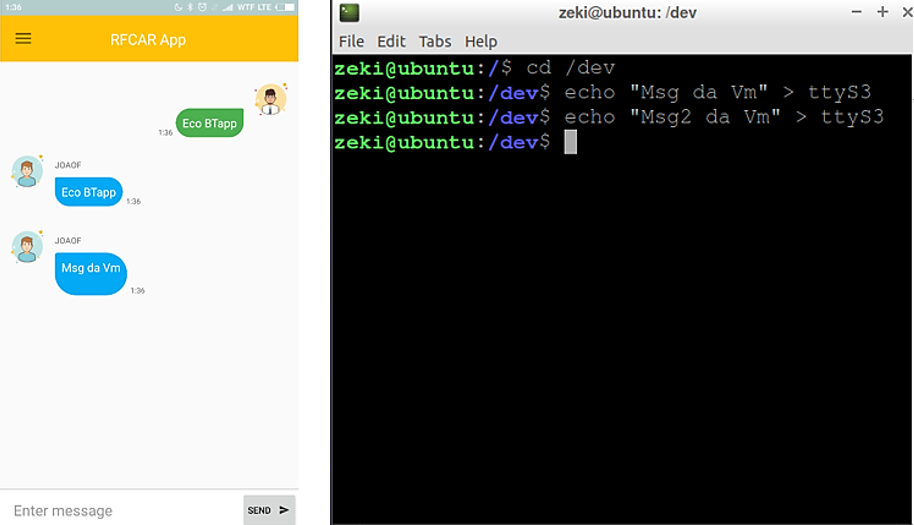
\includegraphics[width=0.5\textwidth]{img/bt_sendPC_recAPP.png}
\caption{\label{fig:bt_sendPC_recAPP}BTapp and PC BT server: Successfull message exchanged from pc to android}
\end{figure}
%
\begin{figure}[!hbt]
\centering

\includegraphics[width=0.3\textwidth]{img/bt_resending_rereceiving.png}
\caption{\label{fig:bt_resending_rereceiving}BTapp: It's possible to resend and receive more than once}
\end{figure}
%
When on the connection setup phase, the scan button was clicked to show the PC to connect as a discoverable device and following that, that same device detected was clicked to pair up with the smartphone. When the pairing phase is completed, one out of two outputs happen. The PC device pairs, as proven in last capture of figure \ref{fig:bt_con_scan_pair_suc}, or doesn't as depicted in figure \ref{fig:bt_failed_pair}, as an example. Error messages would pop up whether the PIN introduced on the PC was mismatched or it was already paired in the first place, accordingly. On the former alternative, the connection was possible after pressing list devices button and clicking on the same target device as when pairing, sequence of events displayed in figure \ref{fig:bt_sequence_connect}.

Lastly, after opening output log terminals to receive app messages on the personal computer virtual machine guest operative system, on the principal menu, in the Enter message section, the messages were typed and then sent via clicking the adjacent send button. The message was then echoed on the phone and conveyed to the target (JOAO F) device, where they were displayed. Figure \ref{fig:bt_sendapp_recpc} show app and PC terminal points of view. Regarding figure \ref{fig:bt_sendPC_recAPP}, the message was written on the terminal and received on the smartphone, respectively. Figure \ref{fig:bt_resending_rereceiving} display final state on the app log after resending a different message as well as obtaining another one via the same source. Note that the PC terminal images already depicts all messages exchanged and show the initial command configuration needed for the test to happen.

On one hand, in the receiving terminal, the first command: \textit{$cd$} \textit{$/media/sf\_ze\_bt\_server$}
changed the directory to where the server app is located. The second: \textit{$make$} \textit{$all$} \textit{$\&\&$ $./com\_ll$} compile all the source files and run \textit{$com\_ll$}.

On the other hand, in the sending terminal, the current directory was changed to \textit{\textit{$/dev$}} with the command: \textit{$cd$} \textit{$/dev$}
to navigate to where virtual COM4 (ttyS3) so that messages could be sent through, as exemplified in the instruction: \textit{$echo$ $Msg$ $da$ $VM$} \textit{$> ttyS3$}. 
%%% Local Variables:
%%% mode: latex
%%% TeX-master: "../../../dissertation"
%%% End:

\subsubsection{UI}%
\label{sec:user-interface}
In the beginning, an app \gls{ui} was initially thought out and made a first test design.
When the user opens the program, the image of the RFCAR appears along with a built-in set of features. It is then explained the vehicle purpose as a navigation tool through inhospitable environments.
%
Following that, on the top left corner, there's a button that when pressed it redirects to the main app activity allowing first-person vision on the controlled car just like a simulated car game, only this time in a real-life scenario. Some statistics, such as the transport position and its velocity, appear in front of full-screen video capture.
%
From that point on, one can also choose to see the map and possibly the route traced along with some more detailed statistics of the remote control car. This first \gls{ui} idea is depicted in figure \ref{fig:first-ui-idea}. Later, some \gls{ui} tests were made in terms of app functionality. One had to make sure the application behaved properly without crashing when, for example, the user intends to rotate the screen. Some activities' (app screens) orientation was fixed to ensure correct behaviour. The ones where that wasn't an issue, a version for landscape was created and tested (figure \ref{fig:orientation-test}). 
%
\begin{figure}[!ht]
\centering
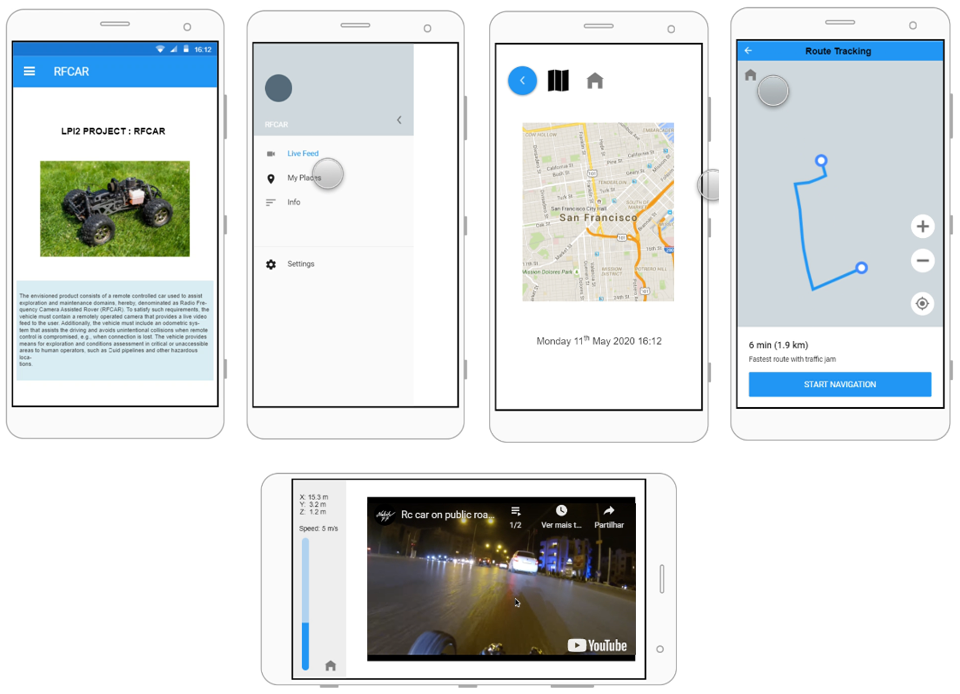
\includegraphics[width=0.8\textwidth]{img/Initial-app-idea.png}
\caption{\label{fig:first-ui-idea}First UI idea}
\end{figure}
%
\begin{figure}[!ht]
\centering
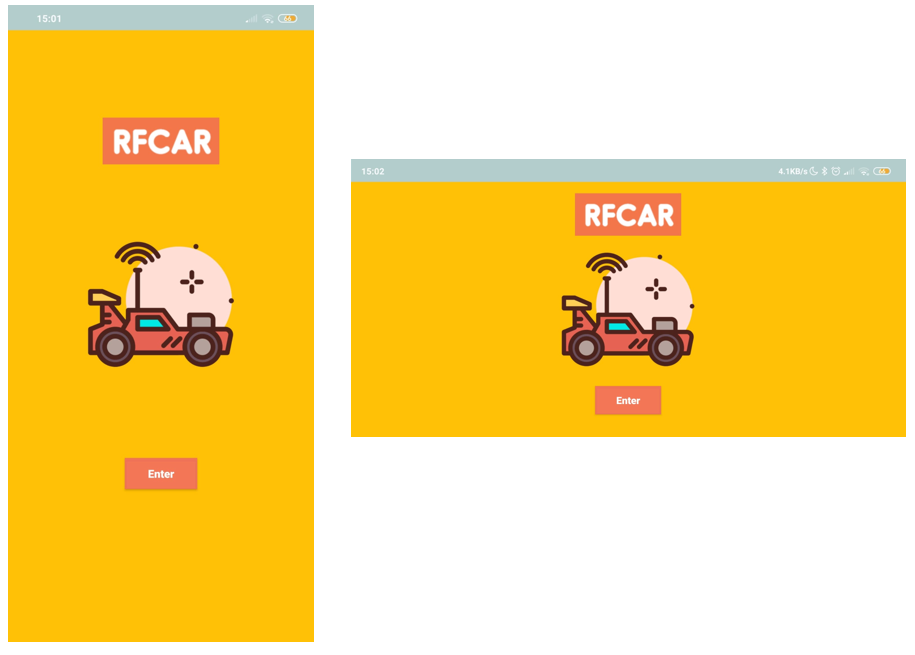
\includegraphics[width=0.8\textwidth]{img/orientation-test.png}
\caption{\label{fig:orientation-test}UI orientation test example}
\end{figure}
%%% Local Variables:
%%% mode: latex
%%% TeX-master: "../../../dissertation"
%%% End:
\subsubsection{Applying Accelerometer Data}
\label{sec:accelerometer-using-data-test}
%
\subsubsection{Message Exchange}
\label{sec:bt-connection-test}
%
    %
\section{Integrated testing}%
\label{sec:integrated-testing}
%\input{./tex/Chap/Testing/unit-testing}
%
%
%%% Local Variables:
%%% mode: latex
%%% TeX-master: "../../../dissertation"
%%% End:
